\documentclass[letterpaper,12pt]{article}

\usepackage{graphicx}                                        
\usepackage{amssymb}                                         
\usepackage{amsmath}                                         
\usepackage{amsthm}                                          

\usepackage{alltt}                                           
\usepackage{float}
\usepackage{color}
\usepackage{url}

\usepackage{balance}
\usepackage[TABBOTCAP, tight]{subfigure}
\usepackage{enumitem}
\usepackage{pstricks, pst-node}

\usepackage{geometry}
\geometry{textheight=8.5in, textwidth=6in}

\newcommand{\cred}[1]{{\color{red}#1}}
\newcommand{\cblue}[1]{{\color{blue}#1}}

\newcommand{\toc}{\tableofcontents}

\usepackage{hyperref}

\def\name{Drake Bridgewater}
\def\title{Assignment 1}
\def\subtitle{}
\def\subject{MTH }
\def\courseNumber{ 351 }
\def\courseName{Numerical Analysis}
\def\courseInfo{Spring 2014 }%Class Time: MWF X-X:XX AM}
\def\supervisor{Thomas \textsc{Hemphries}} % Supervisor's Name


%pull in the necessary preamble matter for pygments output
%\input{pygments.tex}

%% The following metadata will show up in the PDF properties
 \hypersetup{
   colorlinks = false,
   urlcolor = black,
   pdfauthor = {\name},
   pdfkeywords = {\title, \subject, \courseNumber, \courseName, \supervisor},
   pdftitle = {\title},
   pdfsubject = {\subject},
   pdfpagemode = UseNone
 }

\parindent = 0.0 in
\parskip = 0.1 in

\begin{document}


\begin{titlepage}

\newcommand{\HRule}{\rule{\linewidth}{0.5mm}} % Defines a new command for the horizontal lines, change thickness here

\center % Center everything on the page
 
%----------------------------------------------------------------------------------------
%        HEADING SECTIONS
%----------------------------------------------------------------------------------------

\textsc{\LARGE Oregon State University}\\[1.5cm] % Name of your university/college
\textsc{\Large \subject \courseNumber - \courseName}\\[0.5cm] % Major heading such as course name
\textsc{\large \courseInfo}\\[0.5cm] % Minor heading such as course title

%----------------------------------------------------------------------------------------
%        TITLE SECTION
%----------------------------------------------------------------------------------------

\HRule \\[0.4cm]
{ \huge \bfseries \title }\\[0.4cm] % Title of your document
{\small \textit{\subtitle}}\\[0.4cm]
\HRule \\[1.5cm]
 
%----------------------------------------------------------------------------------------
%        AUTHOR SECTION
%----------------------------------------------------------------------------------------

\begin{minipage}{0.4\textwidth}
\begin{flushleft} \large
\emph{Author:}\\
\name
\end{flushleft}
\end{minipage}
~
\begin{minipage}{0.4\textwidth}
\begin{flushright} \large
\emph{Professor:} \\
\supervisor
\end{flushright}
\end{minipage}\\[4cm]

% If you don't want a supervisor, uncomment the two lines below and remove the section above
%\Large \emph{Author:}\\
%John \textsc{Smith}\\[3cm] % Your name

%----------------------------------------------------------------------------------------
%        DATE SECTION
%----------------------------------------------------------------------------------------

{\large \today}\\[3cm] % Date, change the \today to a set date if you want to be precise

%----------------------------------------------------------------------------------------
%        LOGO SECTION
%----------------------------------------------------------------------------------------

%\includegraphics{Logo}\\[1cm] % Include a department/university logo - this will require the graphicx package
 
%----------------------------------------------------------------------------------------

\vfill % Fill the rest of the page with whitespace

\end{titlepage}

%\tableofcontents
%\vfill % Fill the rest of the page with whitespace
%\newpage


\section{Cancellation Error} 

\subsection*{a} $log(x+1)-log(x)$ can be rewritten to $log(1+x/1)$ using basic log properties to avoid cancellation error near x values of -.5 and you get overflow error around$>100,000$
\subsection*{b}$\sqrt{1+\dfrac{1}{x}}-1$
\subsection*{c}$\dfrac{x-sin(x)}{x^3}$ can be separated into to fractional parts leaving $\dfrac{1}{x^2} - \dfrac{sin(x)}{x^3}$ to eliminate the cancellation errors

\section{Eigenvalues}
\subsection*{a}Compute the eigenvalues of 
$\begin{bmatrix}
 1 & 10^6 \\
  0 & 1 
\end{bmatrix}$? The eigenvalues are 1 and 1\\
Compute the eigenvalues of 
$\begin{bmatrix}
 1 & 10^6 \\
  10^{-6} & 1 
\end{bmatrix}$? The eigenvalues are 2 and 0\\
How large is the change in the result compared to the change from matrix one to the other? They are $10^6$ apart
\subsection*{b}Compute the eigenvalues of 
$\begin{bmatrix}
 1 & 2 \\
  0 & 3 
\end{bmatrix}$? The eigenvalues are 1 and 3\\
Compute the eigenvalues of 
$\begin{bmatrix}
 1 & 2 \\
  10^{-6} & 3 
\end{bmatrix}$? The eigenvalues are 1 and 3\\
What can you conclude about the conditioning of problem b verses problem a? I can conclude that the problem a has not been well conditioned therefor it is more sensitive to input changes


\section{Unstable Recursion}
\subsection*{a}
What can you say about the value of the integral $I_n$ as $n$ increases?\\
What is the limit as $n\rightarrow\infty$?\\
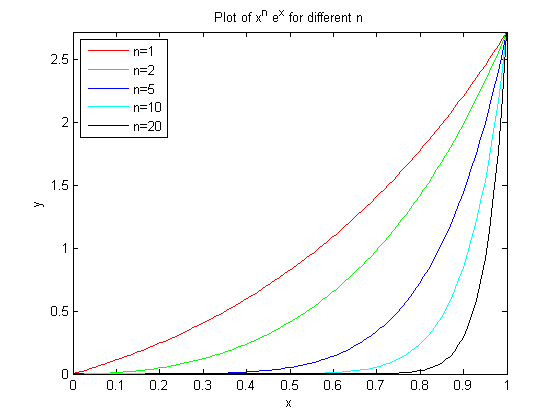
\includegraphics[]{integralPlot.png}
\newpage
\subsection*{b} Prove the following recursive identity using integration by parts:
\[I_0 = e-1\]

\begin{flushright}
$\begin{matrix}
u=e & v'=-1\\
u'=e &v= -x+c
\end{matrix}$
\end{flushright}
\[\int^1_0x^ne^x dx = \left[ x^ne^x-\int e^x x^{n-1}\right[^1_0\]

\[I_{n+1}=e-nI_n\]

\newpage
\subsection*{c}Implement the recursive formula from (b) in matlab. Do the values appear correct? They appear incorrect as the values do not continuously decrease. 
\begin{verbatim}
   I=exp(1)-1;
   for n = 1:25
        I_new = exp(1) - n*I(end);
        I = [I I_new];   % sticks new value on end of array using concatenation
   end
   fprintf('   n \t  I_n \n-------\t--------\n');
   fprintf('   %d\t%7.6f \n',[0:25; I]);
RESULTS
   n 	  I_n 
-------	--------
   0	1.718282 
   1	1.000000 
   2	0.718282 
   3	0.563436 
   4	0.464536 
   5	0.395600 
   6	0.344685 
   7	0.305490 
   8	0.274362 
   9	0.249028 
   10	0.228002 
   11	0.210265 
   12	0.195100 
   13	0.181982 
   14	0.170533 
   15	0.160282 
   16	0.153766 
   17	0.104254 
   18	0.841710 
   19	-13.274218 
   20	268.202632 
   21	-5629.536995 
   22	123852.532175 
   23	-2848605.521754 
   24	68366535.240386 
   25	-1709163378.291363 
\end{verbatim}
\subsection*{d}
Explain part c? Not sure but it will have to deal with machine epsilon
\subsection*{e}
\begin{verbatim}
I = 0;%ENTER STARTING VALUE FOR I HERE

for n = 50:-1:1
    %ENTER BACKWARD RECURSIVE FORMULA HERE
    I_new = 
    
    
    I = [I_new I];          % This sticks the new value on the 
                            %  BEGINNING of the array using concatenation. 
                            % access the first element of array with I(1).
end

fprintf('   n \t  I_n \n-------\t--------\n');
fprintf('   %d\t%7.6f \n',[0:50; I]);
\end{verbatim}
\subsection*{f}
Explain the results of part (e) versus part (c), in terms of what happens to the numerical error at each step. 



\end{document}